\begin{figure}[H]
    \centering
    \begin{tabular}{|c|}
        \hline
        idx \\
        \hline
    \end{tabular} : case libre
    \begin{tabular}{|c|}
        \hline
        \cellcolor{gray}\color{white}idx \\
        \hline
    \end{tabular} : pion
    \begin{tabular}{|c|}
        \hline
        \cellcolor{green}\color{black}idx \\
        \hline
    \end{tabular} : pièce à jouer
    \\
    \subfloat[Grille de jeu]{
        \begin{tabular}{|c|c|c|c|c|}
            \hline
            0                               & \cellcolor{gray}\color{white}1 & 2                              \\\hline
            \cellcolor{gray}\color{white}3  & 4                              & \cellcolor{gray}\color{white}5 \\\hline
            \cellcolor{green}\color{black}6 & \cellcolor{gray}\color{white}7 & 8                              \\\hline
        \end{tabular}
    }
    \\
    \raisebox{-0.5\height}{
        \subfloat[Arbre des mouvements possibles]{
            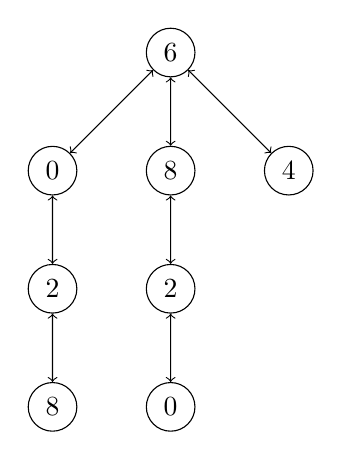
\begin{tikzpicture}[nodes={draw, circle}]
                \node {6}
                child {
                        node {0} edge from parent [<->]
                        child {
                                node {2} edge from parent [<->]
                                child {
                                        node {8} edge from parent [<->]
                                    };
                            };
                    }
                child {
                    node {8} edge from parent [<->]
                    child {
                        node {2} edge from parent [<->]
                        child {
                            node {0} edge from parent [<->]
                        };
                    };
                }
                child {node {4} edge from parent [<->]};
            \end{tikzpicture}
        }
    }
    \hspace{1.5em}
    \raisebox{-0.5\height}{
        \subfloat[Ensemble des mouvements possibles]{
            \begin{tabular}{ ccccccccc }
                0 & 1 & 2 & 3 & 4 & 5 & 6 & 7 & 8 \\\hline
                \multicolumn{1}{|c|}{1}
                & \multicolumn{1}{|c|}{0} 
                & \multicolumn{1}{|c|}{1} 
                & \multicolumn{1}{|c|}{0} 
                & \multicolumn{1}{|c|}{1} 
                & \multicolumn{1}{|c|}{0} 
                & \multicolumn{1}{|c|}{0} 
                & \multicolumn{1}{|c|}{0} 
                & \multicolumn{1}{|c|}{1} 
                \\\hline
            \end{tabular}
        }
    }
    \caption{Deux représentations des mouvements possibles pour un pion}
    \label{fig:example-moves}
\end{figure}